%% (Master) Thesis template
% Template version used: v1.4
%
% Largely adapted from Adrian Nievergelt's template for the ADPS
% (lecture notes) project.


%% We use the memoir class because it offers a many easy to use features.
\documentclass[11pt,a4paper]{memoir}

%% Packages
%% ========

%% LaTeX Font encoding -- DO NOT CHANGE
\usepackage[OT1]{fontenc}

%% Babel provides support for languages.  'english' uses British
%% English hyphenation and text snippets like "Figure" and
%% "Theorem". Use the option 'ngerman' if your document is in German.
%% Use 'american' for American English.  Note that if you change this,
%% the next LaTeX run may show spurious errors.  Simply run it again.
%% If they persist, remove the .aux file and try again.
\usepackage[english]{babel}

%% Input encoding 'utf8'. In some cases you might need 'utf8x' for
%% extra symbols. Not all editors, especially on Windows, are UTF-8
%% capable, so you may want to use 'latin1' instead.
\usepackage[utf8]{inputenc}

%% This changes default fonts for both text and math mode to use Herman Zapfs
%% excellent Palatino font.  Do not change this.
\usepackage[sc]{mathpazo}

%% The AMS-LaTeX extensions for mathematical typesetting.  Do not
%% remove.
\usepackage{amsmath,amssymb,amsfonts,mathrsfs}

%% NTheorem is a reimplementation of the AMS Theorem package. This
%% will allow us to typeset theorems like examples, proofs and
%% similar.  Do not remove.
%% NOTE: Must be loaded AFTER amsmath, or the \qed placement will
%% break
\usepackage[amsmath,thmmarks]{ntheorem}

%% LaTeX' own graphics handling
\usepackage{graphicx}

%% We unfortunately need this for the Rules chapter.  Remove it
%% afterwards; or at least NEVER use its underlining features.
\usepackage{soul}

%% This allows you to add .pdf files. It is used to add the
%% declaration of originality.
\usepackage{pdfpages}

%% Some more packages that you may want to use.  Have a look at the
%% file, and consult the package docs for each.
%% See the TeXed file for more explanations

%% [OPT] Multi-rowed cells in tabulars
%\usepackage{multirow}

%% [REC] Intelligent cross reference package. This allows for nice
%% combined references that include the reference and a hint to where
%% to look for it.
\usepackage{varioref}

%% [OPT] Easily changeable quotes with \enquote{Text}
%\usepackage[german=swiss]{csquotes}

%% [REC] Format dates and time depending on locale
\usepackage{datetime}

%% [OPT] Provides a \cancel{} command to stroke through mathematics.
%\usepackage{cancel}

%% [NEED] This allows for additional typesetting tools in mathmode.
%% See its excellent documentation.
\usepackage{mathtools}

%% [ADV] Conditional commands
%\usepackage{ifthen}

%% [OPT] Manual large braces or other delimiters.
%\usepackage{bigdelim, bigstrut}

%% [REC] Alternate vector arrows. Use the command \vv{} to get scaled
%% vector arrows.
\usepackage[h]{esvect}

%% [NEED] Some extensions to tabulars and array environments.
\usepackage{array}

%% [OPT] Postscript support via pstricks graphics package. Very
%% diverse applications.
%\usepackage{pstricks,pst-all}

%% [?] This seems to allow us to define some additional counters.
%\usepackage{etex}

%% [ADV] XY-Pic to typeset some matrix-style graphics
%\usepackage[all]{xy}

%% [OPT] This is needed to generate an index at the end of the
%% document.
%\usepackage{makeidx}

%% [OPT] Fancy package for source code listings.  The template text
%% needs it for some LaTeX snippets; remove/adapt the \lstset when you
%% remove the template content.
\usepackage{listings}
\lstset{language=TeX,basicstyle={\normalfont\ttfamily}}

%% [REC] Fancy character protrusion.  Must be loaded after all fonts.
\usepackage{microtype}

%% [REC] Nicer tables.  Read the excellent documentation.
\usepackage{booktabs}

\usepackage{csquotes}

\usepackage{xcolor}

\usepackage{colortbl}

\usepackage{tikz}

\usepackage{enumitem}

\usepackage{caption}


%% Make document internal hyperlinks wherever possible. (TOC, references)
%% This MUST be loaded after varioref, which is loaded in 'extrapackages'
%% above.  We just load it last to be safe.
\usepackage[linkcolor=black,colorlinks=true,citecolor=black,filecolor=black]{hyperref}

%% Our layout configuration.  DO NOT CHANGE.
%% Memoir layout setup

%% NOTE: You are strongly advised not to change any of them unless you
%% know what you are doing.  These settings strongly interact in the
%% final look of the document.

% Dependencies
\usepackage{ETHlogo}

% Turn extra space before chapter headings off.
\setlength{\beforechapskip}{0pt}

\nonzeroparskip
\parindent=0pt
\defaultlists

% Chapter style redefinition
\makeatletter

\if@twoside
  \pagestyle{Ruled}
  \copypagestyle{chapter}{Ruled}
\else
  \pagestyle{ruled}
  \copypagestyle{chapter}{ruled}
\fi
\makeoddhead{chapter}{}{}{}
\makeevenhead{chapter}{}{}{}
\makeheadrule{chapter}{\textwidth}{0pt}
\copypagestyle{abstract}{empty}

\makechapterstyle{bianchimod}{%
  \chapterstyle{default}
  \renewcommand*{\chapnamefont}{\normalfont\Large\sffamily}
  \renewcommand*{\chapnumfont}{\normalfont\Large\sffamily}
  \renewcommand*{\printchaptername}{%
    \chapnamefont\centering\@chapapp}
  \renewcommand*{\printchapternum}{\chapnumfont {\thechapter}}
  \renewcommand*{\chaptitlefont}{\normalfont\huge\sffamily}
  \renewcommand*{\printchaptertitle}[1]{%
    \hrule\vskip\onelineskip \centering \chaptitlefont\textbf{\vphantom{gyM}##1}\par}
  \renewcommand*{\afterchaptertitle}{\vskip\onelineskip \hrule\vskip
    \afterchapskip}
  \renewcommand*{\printchapternonum}{%
    \vphantom{\chapnumfont {9}}\afterchapternum}}

% Use the newly defined style
\chapterstyle{bianchimod}

\setsecheadstyle{\Large\bfseries\sffamily}
\setsubsecheadstyle{\large\bfseries\sffamily}
\setsubsubsecheadstyle{\bfseries\sffamily}
\setparaheadstyle{\normalsize\bfseries\sffamily}
\setsubparaheadstyle{\normalsize\itshape\sffamily}
\setsubparaindent{0pt}

% Set captions to a more separated style for clearness
\captionnamefont{\sffamily\bfseries\footnotesize}
\captiontitlefont{\sffamily\footnotesize}
\setlength{\intextsep}{16pt}
\setlength{\belowcaptionskip}{1pt}

% Set section and TOC numbering depth to subsection
\setsecnumdepth{subsection}
\settocdepth{subsection}

%% Titlepage adjustments
\pretitle{\vspace{0pt plus 0.7fill}\begin{center}\HUGE\sffamily\bfseries}
\posttitle{\end{center}\par}
\preauthor{\par\begin{center}\let\and\\\Large\sffamily}
\postauthor{\end{center}}
\predate{\par\begin{center}\Large\sffamily}
\postdate{\end{center}}

\def\@advisors{}
\newcommand{\advisors}[1]{\def\@advisors{#1}}
\def\@department{}
\newcommand{\department}[1]{\def\@department{#1}}
\def\@thesistype{}
\newcommand{\thesistype}[1]{\def\@thesistype{#1}}

\renewcommand{\maketitlehooka}{\noindent\ETHlogo[2in]}

\renewcommand{\maketitlehookb}{\vspace{1in}%
  \par\begin{center}\Large\sffamily\@thesistype\end{center}}

\renewcommand{\maketitlehookd}{%
  \vfill\par
  \begin{flushright}
    \sffamily
    \@advisors\par
    \@department, ETH Z\"urich
  \end{flushright}
}

\checkandfixthelayout

\setlength{\droptitle}{-48pt}

\makeatother

% This defines how theorems should look. Best leave as is.
\theoremstyle{plain}
\setlength\theorempostskipamount{0pt}

%%% Local Variables:
%%% mode: latex
%%% TeX-master: "thesis"
%%% End:


%% Theorem environments.  You will have to adapt this for a German
%% thesis.
%% Theorem-like environments

%% This can be changed according to language. You can comment out the ones you
%% don't need.

\numberwithin{equation}{chapter}

\def\algorithmautorefname{Algorithm}
\def\conjectureautorefname{Conjecture}
\def\corollaryautorefname{Corollary}
\def\definitionautorefname{Definition}
\def\exampleautorefname{Example}
\def\lemmaautorefname{Lemma}
\def\observationautorefname{Observation}
\def\propositionautorefname{Proposition}
\def\remarkautorefname{Remark}
\def\theoremautorefname{Theorem}

\makeatletter
\renewtheoremstyle{plain}%
{\item[\hskip\labelsep \theorem@headerfont ##1\ ##2 \theorem@separator]}%
{\item[\hskip\labelsep \theorem@headerfont ##1\ ##2\ \normalfont{(##3)}  \theorem@separator]}
\makeatother

%% English variants
\theorembodyfont{\normalfont}
\newtheorem{theorem}{\theoremautorefname}[chapter]
\newtheorem{conjecture}{\conjectureautorefname}
\newtheorem{corollary}{\corollaryautorefname}
\newtheorem{definition}{\definitionautorefname}
\newtheorem{example}{\exampleautorefname}
\newtheorem{lemma}{\lemmaautorefname}
\newtheorem{observation}{\observationautorefname}
\newtheorem{proposition}{\propositionautorefname}
\newtheorem{remark}{\remarkautorefname}

%% Proof environment with a small square as a "qed" symbol
\theoremstyle{nonumberplain}
\theorembodyfont{\normalfont}
\theoremsymbol{\ensuremath{\square}}
\newtheorem{proof}{Proof}
%\newtheorem{beweis}{Beweis}


%% Helpful macros.
%% Custom commands
%% ===============

%% Special characters for number sets, e.g. real or complex numbers.
\newcommand{\C}{\mathbb{C}}
\newcommand{\K}{\mathbb{K}}
\newcommand{\N}{\mathbb{N}}
\newcommand{\Q}{\mathbb{Q}}
\newcommand{\R}{\mathbb{R}}
\newcommand{\Z}{\mathbb{Z}}
\newcommand{\X}{\mathbb{X}}

%% Special characters for vectors.
\newcommand\vecs{\boldsymbol{\mathit{s}}}
\newcommand\vect{\boldsymbol{\mathit{t}}}
\newcommand\mm{\boldsymbol{\mathit{m}}}
\newcommand\uu{\boldsymbol{\mathit{u}}}
\newcommand\ppi{\boldsymbol{\pi}}

%% Fixed/scaling delimiter examples (see mathtools documentation)
\DeclarePairedDelimiter\abs{\lvert}{\rvert}
\DeclarePairedDelimiter\norm{\lVert}{\rVert}

%% Use the alternative epsilon per default and define the old one as \oldepsilon
\let\oldepsilon\epsilon
\renewcommand{\epsilon}{\ensuremath\varepsilon}

%% Also set the alternate phi as default.
\let\oldphi\phi
\renewcommand{\phi}{\ensuremath{\varphi}}

\addto\extrasenglish{
  \renewcommand{\chapterautorefname}{Chapter}
  \renewcommand{\sectionautorefname}{Section}
}



%% Document information
%% ====================

\title{Training People for Non-Nashian Thinking}
\author{Martin Kučera}
\thesistype{Practical Work}
\advisors{Supervisors: Dr. Ghislain Fourny, 	Prof. Dr. Thomas Hofmann, Prof. Dr. Manu Kapur}
\department{Department of Computer Science}
\date{January 19, 2038}

\begin{document}

\frontmatter

%% Title page is autogenerated from document information above.  DO
%% NOT CHANGE.
\begin{titlingpage}
  \calccentering{\unitlength}
  \begin{adjustwidth*}{\unitlength-24pt}{-\unitlength-24pt}
    \maketitle
  \end{adjustwidth*}
\end{titlingpage}

%% The abstract of your thesis.  Edit the file as needed.
\begin{abstract}
  This example thesis briefly shows the main features of our thesis
  style, and how to use it for your purposes.
\end{abstract}


%% TOC with the proper setup, do not change.
\cleartorecto
\tableofcontents
\mainmatter

%% Your real content!
\chapter{Introduction}
In Nashian game theory we ask ourselves, if a rational player knew what the strategies of all opponent players, what strategy would she choose.
It would quite naturally be the strategy that maximizes her own payoff.
A state in which no player would be motivated to change strategy even after knowing the opponents' srategies is called a Nash equilibrium.

Non-Nashian game theory offers a different perspective.
It makes the assumption that each player can perfectly predict the other players' strategies.
Let us think about what this means for an individual player (let's call her Alice).
When thinking about this assumption for the first time, it might seem obvious that Alice should just choose whatever strategy yields the best payoff for her, considering all the opponents' strategies that she correctly predicted, i.e., the Nashian best response.
However, since the other players can also predict perfectly, they would know about this and adapt their strategies accordingly.
Since Alice can predict perfectly, she needs to take this into consideration (and the other players need to take her consideration into theirs, and she needs to take theirs into hers, and so on).

For example, consider the famous Prisonner's dilemma (see \autoref{tab:prisoners-dilemma}).
Suppose that Alice was playing against Bob and predicted that Bob was going to cooperate.
Her Nahian best response would then be to defect.
If she did choose to defect though, Bob would predict it and he would defect as well.
This would lead to a Nash equilibrium (defect, defect).
However, it is not a PTE because Alice knew about this from the begining, and she must have also considered the other case---cooperating.
If Alice cooperated, we can see by the same argument (since the game is symmetric) that Bob would not be motivated to switch from cooperating to defecting.
This is because if he defected, Alice would defect as well, and (cooporate, cooparate) has a strictly better payoff for Bob than (defect, defect).
Thus, both Alice and Bob know that cooperating leads to the best possible payoff for each, and (cooperate, cooperate) indeed is a PTE.

\begin{table}
	\caption{Prisoner's dilemma---a standard example of a game in normal form.
	Two suspects (row- and column-player) are placed in solitary confinement, with no means of communicating with each other.
	Each suspect has two options: either cooperate with the other by remaining silent, or defect by testifying against the other.
	If both suspects remain silent, each of them will serve one year in prison.
	If one defects while the other remains silent, the other will serve three years.
	If both defect, each of them will serve two years.
	}
	\label{tab:prisoners-dilemma}
	\centering
	\begin{tabular}{|c|c|c|}
	  \hline
				& cooperate & defect \\
	  \hline
	  cooperate & -1, -1    & -3, 0  \\
	  \hline
	  defect    & 0, -3     & -2, -2 \\
	  \hline
	\end{tabular}
  \end{table}

Note that Alice and Bob actually never needed to use their predictring ability at all.
Just believing that the other player can predict their strategy was enough to choose an optimal strategy.
This is in fact true for any game, not just for our example \cite{Fourny20}.

In general, games can have multiple PTEs.
However, games without ties (sometimes also called games in general position), if a PTE exists, then it is unique and Pareto-optimal \cite{Fourny20}.

We provide a formal definition of PTE in \autoref{chap:background} but this should be enough to illustrate why it is an interesting concept.
Since game theory has many practical applications, it is interesting to research how or under what conditions players might be motivated to play in a way that leads to everyone reaching as good a payoff as possible.

The goal of this work is twofold:
First, it is to develop a REST API-based backend for playing games that will teach human players to think similarly as Alice and Bob in our example.
That is, it will motivate them to play towards a PTE (or at least to something that is, in some sense, close to a PTE).
We develop a backend that supports playing 2-player randomly generated games against a computer.
The backend is in the form of a web (HTTP) based API server.
Any client can connect to the server and request a new game which the server generates randomly and sends back to the client.
Subsequently, the client can then choose a strategy and send it to the server, which responds with the computer's strategy and the resulting payoff.
The human player is supposed to think that the computer chooses its strategy independently, not knowing the opponent's strategy, even though in reality, it actually does know the opponent's strategy and uses it to choose its own---this is to simulate Perfect Prediction.
All games played through the server are stored in a database together with the results so that they can be analyzed later.

The second goal is to define new notions of best responses that might ultimately lead to a PTE.
The idea here is that even though the computer knows its opponent's strategy and it could just play the Nashian best response to maximize its own utility, it should rather choose some potentially suboptimal strategy, such that a player who plays towards a PTE is better off than one who does not.
This way, it might be possible to train people into non-Nashian thinking.
To this end, we define a perfectly transparent best response, perfectly transparent $i$-best profile, and perfectly transparent $i$-optimal profile.
These three best responses induce three new equilibria: perfectly transparent best response equilibrium, perfectly transparent best profile Equilibrium, and perfectly transparent optimal profile equilibrium.
Furthermore, we analyze large datasets of randomly generated games to find out information about how the relate to each other, and to some other equilibra---most importantly to PTE.

\chapter{Background}
\section{Nashian Game Theory}
Here we introduce some basic notions from algorithmic game theory.
A knowledgable reader may safely skip this section.

We start by defining a game in normal form.
Intuitively, it is a game of $n$ players in which each player $i$ has a set of strategies $S_i$, and the goal is to maximize \textit{utility} by choosing the best strategy $s_i \in S_i$.
A vector of length $n$ in which the $i$\textsuperscript{th} element describes the strategy chosen by player $i$ is called a \textit{strategy profile}.
The utility (somtimes also called payoff) is then determined individually for each player based on the strategy profile.
The game is only played once.
Next, we provide a formal definition.

\begin{definition}[Game in normal form]
  We define a game in normal form as a 3-tuple $G = (P, S, \uu)$ where
  \begin{itemize}
    \item $P = \{1, \dots n\}$ is the set of players,
    \item $S$ = $S_1 \times S_2 \times \dots \times S_n$ is the set of strategy profiles,
    \begin{itemize}
      \item $S_i$ is the set of strategies of player $i \in P$,
    \end{itemize}
    \item $\uu = (u_1, u_2, \dots, u_n)$ is the vector of utility functions,
    \begin{itemize}
      \item $u_i: S \rightarrow \R$ is the utility function for player $i \in P$.
    \end{itemize}
  \end{itemize}
  In this work, we will sometimes refer to games in normal form simply as \enquote{games}.
  This should not lead to confusion as we do not consider any other forms.
\end{definition}

Note that we only consider pure strategies, meaning that each player must choose one strategy deterministically, rather than choosing a probability distribution over multiple strategies (usually called mixed strategies).

Every game in normal form can be captured by an $n$-dimensional matrix with one dimension for each player and one index for every strategy in the strategy set of that player.
Every cell of the matrix contains a vector of utilities for each player for a particular strategy profile.

In this work, we focus solely on 2-player games which can be conveniently displayed as 2-dimensional matrices.
In this case, we usually refer to the players the \textit{row player} and the \textit{column player}.
\autoref{tab:prisoners-dilemma} shows an example of such a matrix.

\begin{table}
  \caption{Prisoner's dilemma---a standard example of a game in normal form.
  Two suspects (row- and column-player) are placed in solitary confinement, with no means of communicating with each other.
  Each suspect has two options: either cooperate with the other by remaining silent, or defect by testifying against the other.
  If both suspects remain silent, each of them will serve one year in prison.
  If one defects while the other remains silent, the other will serve three years.
  If both defect, each of them will serve two years.
  }
  \label{tab:prisoners-dilemma}
  \centering
  \begin{tabular}{|c|c|c|}
    \hline
              & cooperate & defect \\
    \hline
    cooperate & -1, -1    & -3, 0  \\
    \hline
    defect    & 0, -3     & -2, -2 \\
    \hline
  \end{tabular}
\end{table}

Now that we have defined games in normal form, we can introduce some more standard notation.

\begin{definition}
  For a strategy profile $\vecs = (s_1, \dots, s_n) \in S$ we denote $\vecs_{-i} = (s_1, \dots, s_{i-1}, s_{i+1}, \dots, s_n)$, i.e., the vector $\vecs$ with element $s_i$ skipped.
  For a strategy $s_i' \in S_i$ of player $i$ we denote $u_i(s_i', \vecs_{-i}) = u_i(s_1, \dots, s_{i-1}, s_{i'}, s_{i+1}, \dots, s_n)$ the utility of player $i$ for strategy profile $\vecs$ with element $s_i$ replaced by $s_i'$.
\end{definition}

In Nashian game theory, we explore the best strategy for a player, supposing that he knew the strategies that all other players would choose.
This is captured by the notion of best response.

\begin{definition}[Nashian best response]
  For a player $i \in P$, we say a strategy $s_i^* \in S_i$ is a Nashian best response to the strategy profile $\vecs_{-i}$ of his opponents if it satisfies
  \[
    u_i(s_i^*, \vecs_{-i}) \ge u_i(s_i', \vecs_{-i})\ \forall s_i' \in S_i.
  \]
\end{definition}

In the example of Prisoner's dilemma in \autoref{tab:prisoners-dilemma}, the Nashian best response for the row player to \textit{cooperate} is \textit{defect}, and the Nashian best response to \textit{defect} is also \textit{defect}.

Having defined a best response, it is quite natural to ask whether there exists a strategy profile in which each player's strategy is the best response to all other players' strategies.
This is formally called the Nash equilibrium.

\begin{definition}[Nash equilibrium]
  We say a strategy profile $\vecs = (s_1, \dots, s_n)$ is a Nash equilibrium if for every player $i \in P$, strategy $s_i$ is a Nashian best response to $\vecs_{-i}$.
\end{definition}

If we consider mixed strategies, at least one Nash equilibrium always exists~\cite{Nash51}.
However, for pure strategies, it is not always the case.

In the case of prisonner's dilemma, the strategy profile (\textit{defect}, \textit{defect}) is the only Nash equilibrium.
The dilemma in this game is that mutual cooperation would yield a better outcome for both players.
However, from a self-interested perspective, it is not considered a rational choice to cooperate under the Nashian assumptions.
We call this \enquote{better} state (\textit{cooperate}, \textit{cooperate}) Pareto-optimal.

\begin{definition}[Pareto-optimality]
  For a game $G = (P, S, \uu)$, we say a strategy profile $s \in S$ \textit{Pareto-dominates} profile $s' \in S$ if
  \begin{itemize}
    \item no player gets a worse payoff with $s$ than with $s'$: $u_i(s) \ge u_i(s')\ \forall i \in P$, and
    \item at lest one player gets a strictly better payoff with $s$ then with $s'$: $\exists i \in P: u_i(s) > u_i(s')$.
  \end{itemize}
  A strategy profile $s \in S$ is \textit{Pareto-optimal} if there is no profile $s' \in S$ that Pareto-dominates $s$.
\end{definition}

\begin{definition}[Symmetric game]
	We say a game $G = (P, S, \uu)$ is symmetric if there is a common set of strategies $S_c$ shared by all players:
  $S_i = S_c\ \forall i \in P$,
  and there is a common utility function $u_c$ shared by all players:
  $u_i = u_c\ \forall i \in P$.
  The utility only depends on the set of opponents' strategies (not on who is playing them):
  \[
    u_c(s_i, \vecs_{-i}) = u_c(s_i, \ppi_{-i})\ \forall s_i \in S_c, \vecs_{-i} \in S_c^{n-1}, \ppi_{-i} \text{ is a permutation of } \vecs_{-i}.
  \]
\end{definition}

\section{Non-Nashian Game Theory}
\begin{definition}[Minimax rationality]
  TODO
\end{definition}

\begin{definition}[Individual rationality]
  For any game $G = (P, S, \uu)$ we say a strategy profile $\vecs = (s_1, \dots, s_n) \in S$ is \textit{not} individually rational if there is a player $i \in P$ who could, by choosing a different strategy $s_i' \ne s_i$, ensure a higher worst-case payoff (across all possible opponent profiles) than $u_i(\vecs)$.
  Otherwise, we say $\vecs$ is individually rational.
  Formally, a strategy profile $\vecs$ is individually rational if
  \[
    \forall i \in P: u_i(\vecs) \ge \max_{t_i\in S_i}\min_{\vect_{-i} \in S_{-i}}u_i(t_i, \vect_{-i}).
  \]
\end{definition}

\begin{observation}
  A Nash equilibrium is always individually rational.
\end{observation}

While a Nash equilibrium is an outcome that is always individually rational, it might not be Pareto-optimal (as in the case of Prisoner's dilemma).
A~natural question to ask is whether, under some special conditions, we could ensure that rational players will always end up with a Pareto-optimal strategy profile.
For example, it is known that playing Prisoner's dilemma repeatedly for a fixed number of times (with both players knowing the number) does not motivate rational players to change strategies: each player will defect in every round.
However, when the total number of rounds is not known to the players, defecting in each round may not be a dominant strategy anymore.
For indefinitely long games, rational players can sustain the cooperative outcome.
% https://www.degruyter.com/document/doi/10.1515/9781400882168-018/html
% https://msp.org/pjm/1960/10-2/pjm-v10-n2-p02-p.pdf

Another assumption that one can make in order to change the outcomes drastically is (1) Necessery Knowledge of Strategies and (2) Necessary Rationality, as described by Fourny \cite{Fourny20}.
Informally, this means that
\begin{enumerate}[label=(\arabic*)]
  \item All players can perfectly predict the strategies chosen by their opponents.
  In other words, they know the strategy profile that the game will reach, before it is even played.
  \item All players are rational in all possible worlds.
  In other words, whatever strategy they choose, it maximizes their own utility.
  If one player would have chosen a different strategy, all the others would have known and would still have acted rationally.
\end{enumerate}
Making these two assumptions together allows to define a new kind of equilibrium.
It is based on iteratively eliminating strategy profiles that cannot possibly be an outcome of the game.
First, it is easy to see that any strategy profile that is not individually rational cannot be an outcome of the game because there would be some player who would surely be better off with a different strategy (and the player can predict it because of Necessare Knowledge of Strategies).
Thus, in the first round of elimination, we can eliminate all strategy profiles that are not individually rational.
Now, since every player knows that only individually rational strategy profiles are possible outcomes, they do not actually need to consider the eliminated profiles anymore.
This naturally leads to another round of elimination, in which we only keep profiles that are individually rational with respect to the set of possible outcomes from the previous round.
The iterative process of eliminating impossible strategy profiles is described by the following definition.

\begin{definition}[$k$\textsuperscript{th}-level-preempted strategy profile]
  For a given game $G = (P, S, \uu)$, we define $\mathcal{S}_0(G) = S$.
  For $k \ge 1$, we say a strategy profile is $k$\textsuperscript{th}-level-preempted if it does not Pareto-dominate the maximin utility over all strategy profiles that are not $(k-1)$\textsuperscript{st}-level preempted.
  The set of strategy profiles that survived the $k$\textsuperscript{th} round of elimination is
  \[
    \mathcal{S}_k(G) = \left\{\vecs \in \mathcal{S}_{k-1}(G) \mid \forall i \in P: u_i(\vecs) \ge \max_{t_i \in S_i}\min_{t_{-i} \in S_{-i}} u_i(t_i, t_{-i})\right\}.
  \]
\end{definition}

Finally, we define a perfectly transparent equilibrium, which is the main focus of this work.

\begin{definition}[Perfectly transparent equilibrium]
  For a given game $G = (P, S, \uu)$ with no ties, a perfectly transparent equilibrium (PTE) is a strategy profile $\vecs \in S$ that never gets eliminated in the preemtpion process.
  In other words, $\vecs \in S$ is a PTE if $\vecs \in \mathcal{S}_k(G)\ \forall k \in \N$.
\end{definition}

For any game with no ties, if a PTE exists, then it is unique and Pareto-optimal~\cite{Fourny20}.

\section{Web Development}
\section{Data Analysis}

\chapter{Implementation}
The implementation is divided into several modules: \textit{core} (code for computing different equilibria), \textit{web} (a backend engine that allows to play games and stores the results in a database), \textit{console} (a console client for the web API), \textit{structures} (common structures for \textit{web} and \textit{console}), and \textit{analysis} (Spark code to analyze large datasets of games).
Each module is described in a separate section below.

There are several services ready to be used via Docker Compose, and can simply be run without the need of installing any additional software:
\textit{web} (the web API server), \textit{postgres} (a PostgreSQL database; is started automatically when running \textit{web}), \textit{console} (the console interface), \textit{analysis} (Apache Spark with commands from the \textit{analysis} module made available), and \textit{sbt} (the building tool; can be used to compile modules and to run tests).

\section{Core module}
While the core module does not contain much code, it is the heart of this project.
It defines the following entities:
\begin{itemize}
	\item \textsc{Game}: a case class that represents a game in normal form for two players.
	\item \textsc{BestResponse}: a trait that describes a best response, given a game and the opponent's strategy.
	It provides a method \textit{equilibria} which automatically computes all equilibria induced by the respective best response.
	It is implemented by the following objects:
	\begin{itemize}
		\item \textsc{NashianBestResponse.Weak}
		\item \textsc{NashianBestResponse.Strict}
		\item \textsc{PerfectlyTransparentBestResponse.Weak}
		\item \textsc{PerfectlyTransparentBestResponse.Strict}
	\end{itemize}
	\item \textsc{Eliminator}: a trait that describes an elimination process used for computing equilibria.
	It defines method \textit{eliminate} which represents one round of elimination.
	It implements method \textit{all} which performs the loop of elimination as long as the set of non-eliminated profiles keeps changing.
	It is implemmented by the following objects:
	\begin{itemize}
		\item \textsc{IndividualRationality}
		\item \textsc{MinimaxRationalizability}
	\end{itemize}
	\item In the theoretical part of this work, we also define some other equilibria: PTBPE and PTOPE.
	These are not induced by best response definitions.
	Instead, they are defined as strategy profiles where the \textit{perfectly transparent $i$-best profiles} and \textit{perfectly transparent $i$-optimal profiles} coincide for all players $i$.
	These are implemented by the following objects:
	\begin{itemize}
		\item \textsc{PerfectlyTransparentRowBestProfile.Weak}
		\item \textsc{PerfectlyTransparentRowBestProfile.Strict}
		\item \textsc{PerfectlyTransparentColOptimalProfile.Weak}
		\item \textsc{PerfectlyTransparentColOptimalProfile.Strict}
	\end{itemize}
	\item \textsc{GameGenerator}: an object for generating random games.
\end{itemize}

\section{Web module}
\label{sec:impl-web-module}
The web module is a web server that provides a REST API for playing games in normal form against a computer.
Every time a game is played, the result is stored in a PostgreSQL database (see \autoref{fig:db-schema}).
The API exposes the following endpoints:
\begin{itemize}
	\item \textsc{NewUser}: Creates a new user and returns the user's ID.
	\item \textsc{NewGame}: Starts a new game; returns the game matrix and ID.
	\item \textsc{Play}: For a game with a given ID, accepts the human player's (row) strategy and returns the computer's (column) strategy.
	\item \textsc{Stats}: Returns statistics for a user with a given ID: number of games played and the average payoff.
\end{itemize}

Play Framework is used to implement the server.
For communicating with the database, we use Slick library.

\begin{figure}
	\hspace{-1cm}
	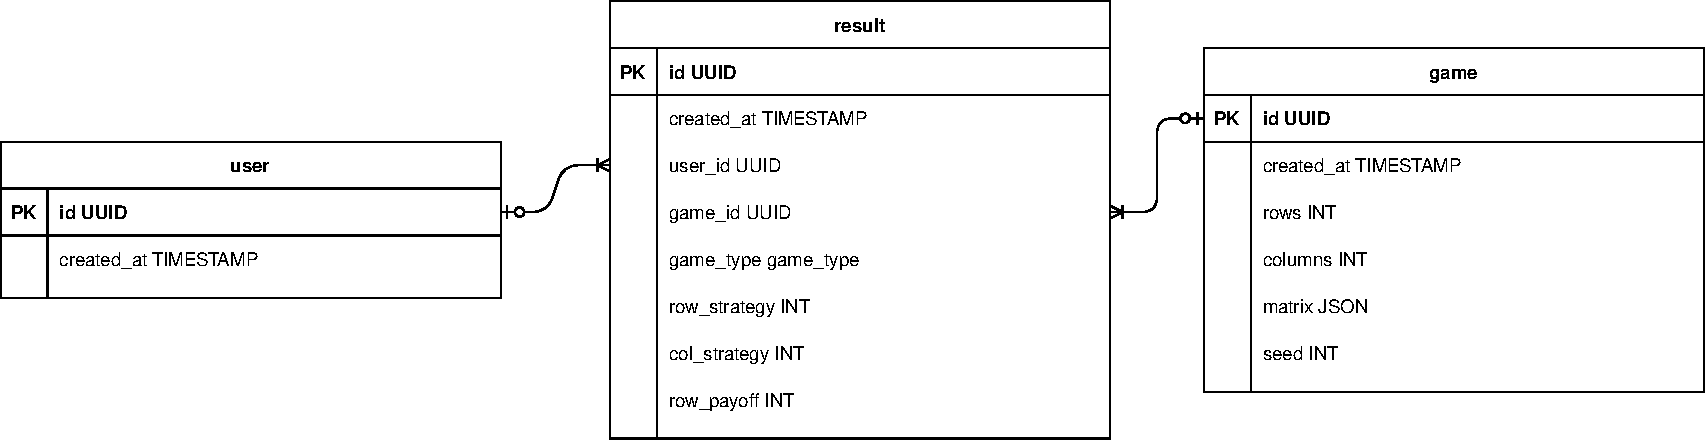
\includegraphics[width=14cm]{fig/schema.pdf}
	\caption{The database schema.}
	\label{fig:db-schema}
\end{figure}

\section{Console module}
The console module is a sample client for the REST API described in \autoref{sec:impl-web-module}.
It allows the user to play a series of games of chosen dimensions.
For each game, the game matrix is displayed, and the user is asked to choose a strategy.
After choosing a strategy, the computer's strategy and the resulting payoff is displayed.
Then, the user is asked whether she wants to play another game.
At the end, statistics over all games are displayed.

\begin{figure}
	\centering
	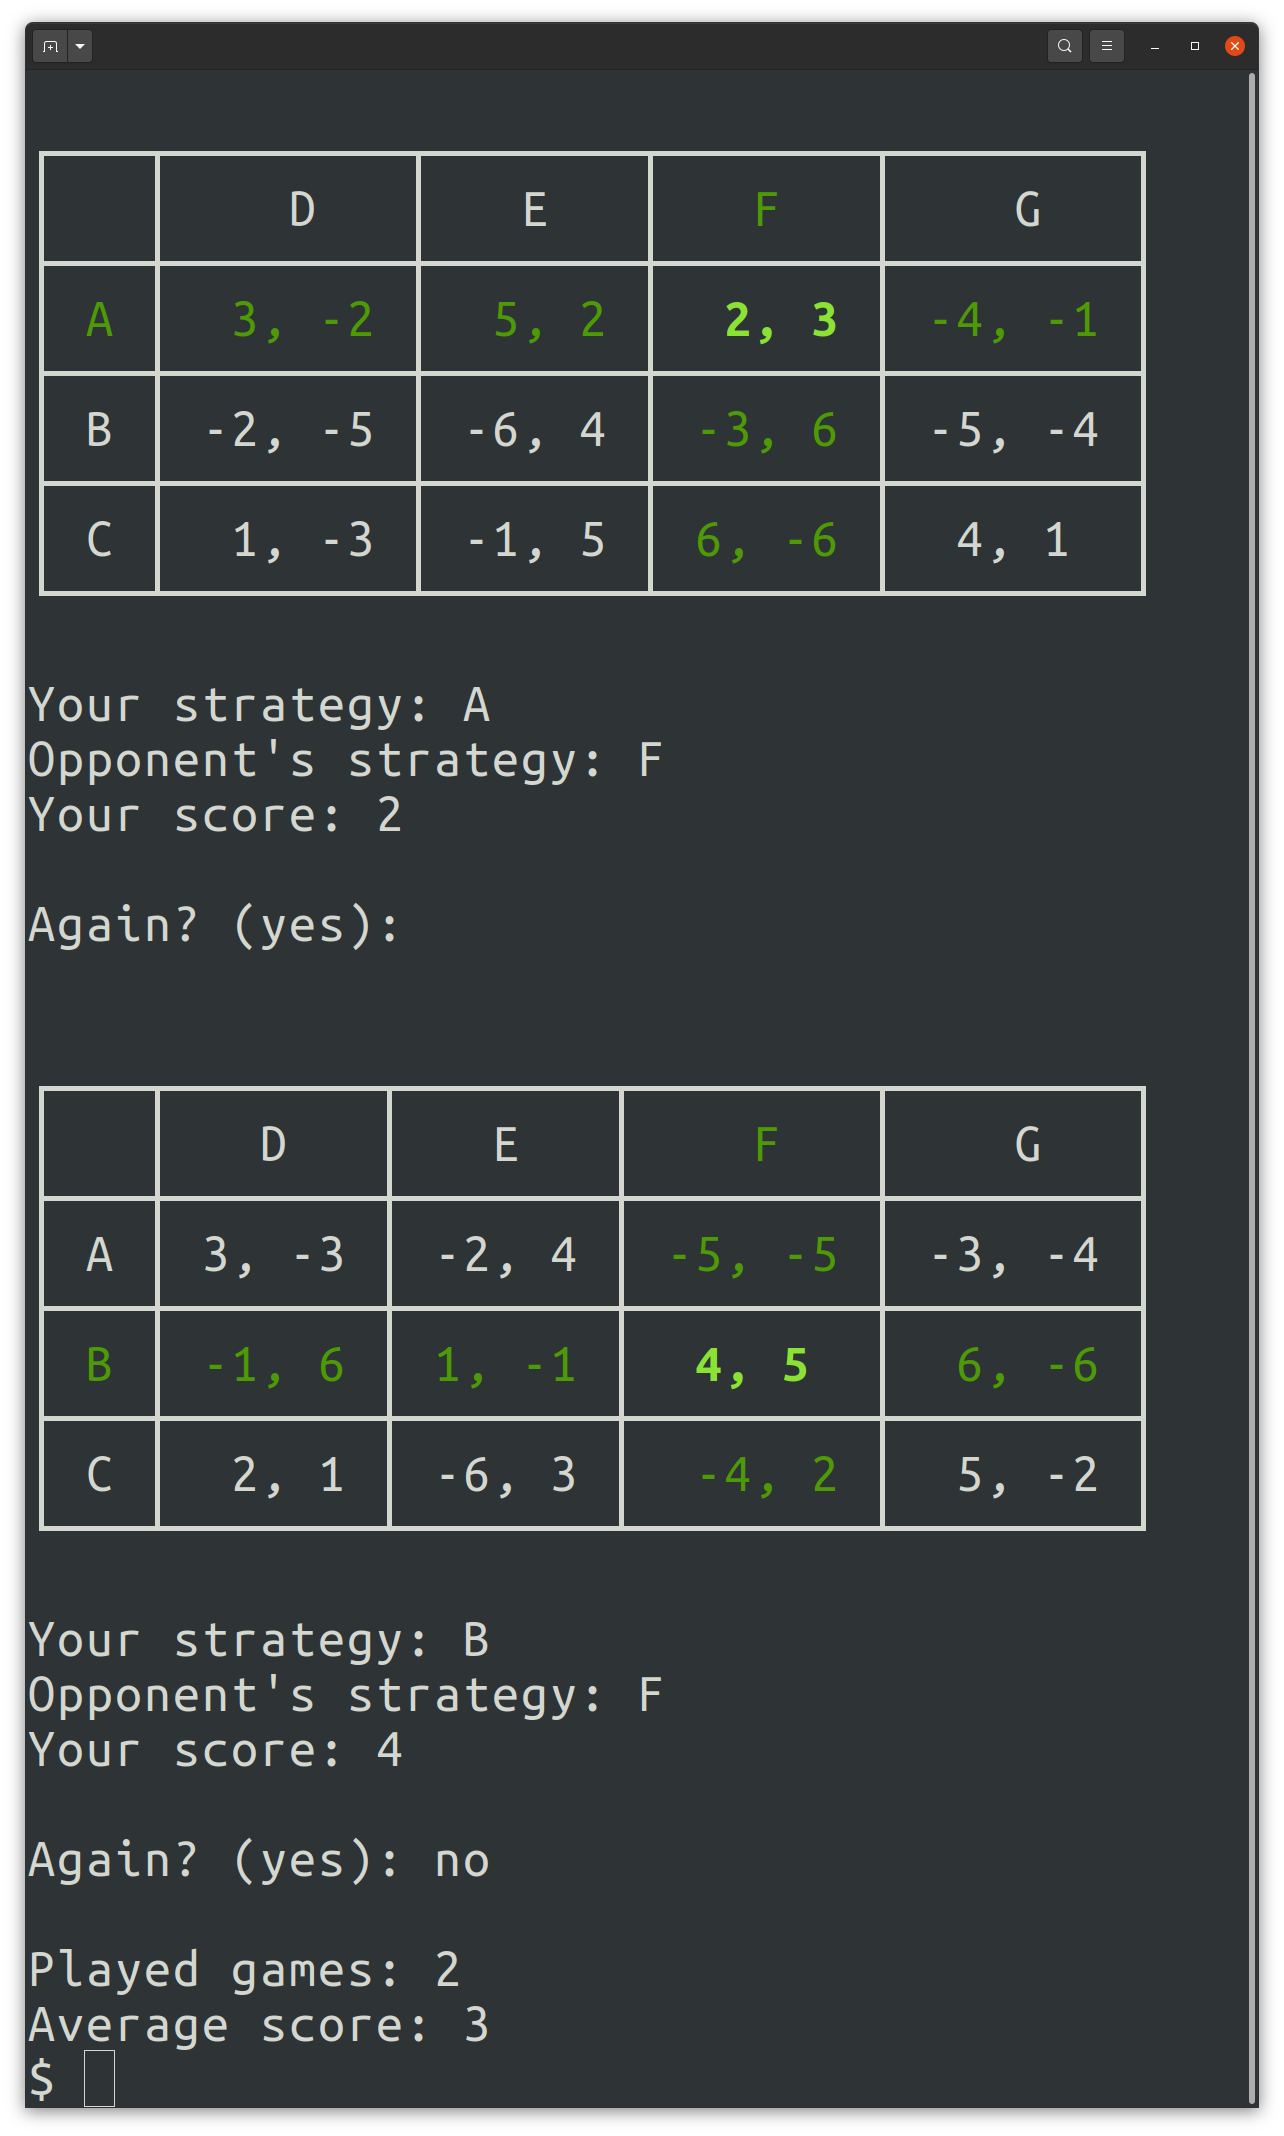
\includegraphics[width=12cm]{fig/console.png}
	\caption{The console interface.}
	\label{fig:console-screen}
\end{figure}

\section{Analysis module}
The analysis module is used for computing statistics about large datasets of games using Apache Spark.
It loads the datasets and computes the PTBPE, PTBRE, individually rational and minimax rationalizable strategy profiles, and stores them as a new dataset.
Searching through this dataset was useful to find counterexamples and form conjectures about inclusions of these equilibria (see \autoref{chap:game-theory}).

\chapter{Game Theory}
\label{chap:game-theory}

\begin{lemma}
	For every game $G$, there exists at least one individually rational strategy profile.
	In other words, $\mathcal{S}_1(G) \ne \emptyset$.
\end{lemma}

\begin{proof}
	For every player $i \in P$ we denote $m_i = \text{arg} \max_{t_i \in S_i} \min_{\vect_{-i} \in S_{-i}} u_i(t_i, \vect_{-i}) \in S_i$ the strategy that lower-bounds utility of player $i$.
	We claim that the strategy profile $\mm = (m_1, \dots, m_n) \in S$ is individually rational.
	If $\mm$ was not individually rational, there would have to be some player $j \in P$ and a strategy $s_j^* \in S_j$ that would ensure a better worst-case payoff: $\min_{\vecs_{-j} \in S_{-j}}u_j(s_j^*, \vecs_{-j}) > u_j(\mm)$ which would contradict the choice of $m_j$.
\end{proof}

\section{Games without ties}

\begin{observation}
	\label{th:pte-subset-ir}
	If a game $G = (P, S, \uu)$ has a PTE $\vecs \in S$, then $\vecs$ is individually rational.
	However, not every individually rational profile is a PTE.
	In other words, if we think of PTE and IR as sets of strategy profiles in any given game, we have PTE $\subsetneq$ IR.
\end{observation}

\begin{definition}[Perfectly transparent best response]
	For a game $G = (P, S, \uu)$ we say a strategy $s_i^* \in S_i$ is a perfectly transparent best response to a strategy profile $\vecs_{-i}$ of the opponent players if it is the Nashian best response to $\vecs_{-i}$ across all profiles that survive the maximum number of preemption rounds before all possible profiles are eliminated.
	Formally, there is some $k \in \N$ such that $(s_i^*, \vecs_{-i}) \in \mathcal{S}_k$, and $(s_i, \vecs_{-i}) \notin \mathcal{S}_{k+1} \forall s_i \in S_i$, and
	\[
		u_i(s_i^*, \vecs_{-i}) \ge u_i(s_i', \vecs_{-i})\ \forall (s_i', \vecs_{-i}) \in \mathcal{S}_k.
	\]
\end{definition}

\begin{definition}[Perfectly transparent best response equilibrium]
	We say a strategy profile $\vecs = (s_1, \dots, s_n) \in S$ is a perfectly transparent best response equilibrium (PTBRE) if $s_i$ is a perfectly transparent best response to $\vecs_{-i}$ for all players $i \in P$.
\end{definition}

\begin{lemma}
	For any game $G = (P, S, \uu)$, if a strategy profile $\vecs \in S$ is a PTBRE, then it is individually rational.
	Thus, we have PTBRE $\subset$ IR.
\end{lemma}

\begin{proof}
	Let us suppose that there is a game $G = (P, S, \uu)$ and a strategy profile $\vecs = (s_1, \dots, s_n) \in S$ such that $\vecs$ is a PTBRE but not individually rational.
	This is equivalent to $s_i$ being a perfectly transparent best response to $\vecs_{-i}$ for all $i \in P$, and $\vecs \notin \mathcal{S}_1$.
	Note that we must also have $(s_i', \vecs_{-i}) \notin \mathcal{S}_1\ \forall s_i' \in S_i,\ \forall i \in P$ because otherwise $s_i$ would not be a perfectly transparent best response to $\vecs_{-i}$ for some player $i$.
	This means the perfetcly transparent best response of every player $i \in P$ to $\vecs_{-i}$ is simply a Nashian best response (since all considered strategy profiles are eliminated in the same preemption round).
	Thus, $\vecs$ is a Nash equilibrium, which is always individually rational.
\end{proof}

\begin{remark}
	\autoref{tab:ir-ne-ptbre} shows that the inclusion is indeed strict.
\end{remark}

\begin{observation}
	\label{th:ptbre-subset-pte}
	If a strategy profile is a PTE, then it must be a PTBRE; we have PTE $\subset$ PTBRE.
\end{observation}

\begin{remark}
	\autoref{tab:ptbre-ne-pte} shows that the inclusion is strict.
\end{remark}

\begin{definition}[Perfectly transparent $i$-best profile]
	For a game $G = (P, S, \uu)$ and player $i \in P$ we say a strategy profile $\vecs = (s_1, \dots, s_n) \in S$ is a perfectly transparent $i$-best profile if
	$s_i$ is a perfectly transparent best response to $\vecs_{-i}$ and $u_i(\vecs) \ge u_i(b(\vecs'_{-i}), \vecs'_{-i})$ for all opponent profiles $\vecs'_{-i}$ where $b(\vecs'_{-i})$ is the perfectly transparent best response to $\vecs'_{-i}$.
\end{definition}

\begin{definition}[Perfectly transparent best profile equilibrium]
	We say a strategy profile $\vecs \in S$ is a perfectly transparent best profile equilibrium (PTBPE) if $\vecs$ is a perfectly transparent $i$-best profile for all $i \in P$.
\end{definition}

\begin{lemma}
	If a game $G = (P, S, \uu)$ has a PTBPE $\vecs \in S$, then $\vecs$ is also a PTE, i.e., we have the inclusion PTBPE $\subset$ PTE.
\end{lemma}

\begin{proof}
	For the sake of deriving a contradiction, suppose that there is a game $G = (P, S, \uu)$ with a strategy profile $\vecs = (s_1, \dots, s_n) \in S$ such that $\vecs$ is a PTBPE but not a PTE and let $k$ be the last preemption round in which $\vecs$ is not eliminated (i.e., $\vecs \in \mathcal{S}_k$ but $\vecs \notin \mathcal{S}_{k+1}$).
	Because $\vecs$ is eliminated in the $(k+1)$\textsuperscript{st} round, there must be some player $i \in P$ with a strategy $s_i^* \ne s_i$ which causes the elimination:
	\[
		\forall \vecs_{-i}' \in S_{-i}: (s_i^*, \vecs_{-i}') \in \mathcal{S}_k \implies u_i(s_i^*, \vecs_{-i}') > u_i(\vecs).
	\]
	Let $\vecs_{-i}^* \in S_{-i}$ such that $(s_i^*, \vecs_{-i}^*)\in \mathcal{S}_k$ (there must be at least one to cause $\vecs \notin \mathcal{S}_{k+1}$).
	We have $u_i(s_i^*, \vecs_{-i}^*) > u_i(\vecs)$ which means $s_i$ is not a perfectly transparent best response of player $i$ to $\vecs_{-i}$, so $\vecs$ is not a perfectly transparent $i$-best profile, contradicting $\vecs$ being a PTBPE.
\end{proof}

\begin{remark}
	\autoref{tab:pte-ne-ptbpe} shows that the inclusion is strict.
\end{remark}

Minimax rationalizibility intersects with all the other equilibiria, as shown in \autoref{tab:ptbpe-ne-minimax} and \autoref{tab:ptbpe-eq-minimax}.

\begin{figure}
	\caption{A venn diagram depicting the inclusion of different equilibria.}
	\centering

	\begin{tikzpicture}[line width=0.25pt]
		\draw (0,0) circle (1);
		\draw (0,0) circle (2);
		\draw (0,0) circle (3);
		\draw[rounded corners=2ex] (-3.5,3.5) rectangle (3.5,-3.5);
		\draw (4.5,0) ellipse (4 and 3);
		\node at (-0.2,0) {PTBPE};
		\node at (-0.2,1.35) {PTE};
		\node at (-0.2,2.35) {PTBRE};
		\node at (-0.2,3.25) {IR};
		\node at (5,0) {MR};
	\end{tikzpicture}
\end{figure}

\section{Symmetric games without ties}

\begin{observation}
	 In a symmetric game $G = (P, S, \uu)$, if a strategy profile $\vecs \in S$ is a PTE, then it lies on the diagonal, i.e., we have $\vecs = (a, a, \dots, a)$ for some strategy $a$.
\end{observation}

\begin{proof}
	If there was a PTE somewhere else than on the diagonal, we would necessarily have multiple PTEs by symmetry, contradicting the uniqueness of PTE.
\end{proof}

\begin{corollary}
	If a symmetric game $G = (P, S, \uu)$ has a PTE $\vecs \in S$ and $\vecs$ is the perfectly transparent $i$-best profile for some player $i \in P$, then $\vecs$ is a PTBPE. 
\end{corollary}

\begin{proof}
	Since $\vecs$ is on the diagonal and it is the perfectly transparent $i$-best profile for some $i \in P$, by symmetry, it must actually be the perfectly transparent $j$-best profile for all $j \in P$, which is the definition of PTBPE.
\end{proof}

\begin{lemma}
	In a symmetric game $G = (P, S, \uu)$, if a strategy profile $\vecs \in S$ is a PTE, then it is minimax rationalizable.
	Thus, we have PTE\textsuperscript{sym} $\subset$ MR.
\end{lemma}

\begin{proof}
	Suppose for the sake of deriving a contradiction that there is a game $G = (P, S, \uu)$ and a strategy profile $\vecs \in S$ that is a PTE but not minimax rationalizable.
	By definition, this means that there is some player $i \in P$ such that $(s_i, \vecs_{-i}')$ is not minimax rationalizable for any $\vecs' \in S$.
	By symmetry, if this statement holds for one player, then it must hold for all players.
	Let $s_j$ be the strategy that minimax-dominates $s_i$ (i.e. causes that $s_i$ is not minimax rationalizable).
	We denote $\vecs^* = (s_j, s_j, \dots, s_j)$.
	In the round where strategy $s_i$ is eliminated, strategy profile $\vecs^*$ must survive---otherwise strategy $s_j$ would be eliminated as well, but we supposed that $s_j$ is the strategy that caused the elimination of $s_i$.
	Moreover, we must have $u_i(\vecs^*) > u_i(\vecs)\ \forall i \in P$ because $s_j$ minimax-dominates $s_i$.
	This means $\vecs$ is not Pareto-optimal which contradicts $\vecs$ being a PTE.
\end{proof}

\chapter{Conclusion}



\appendix

\chapter{Appendix}

\section{Game Theory}
In this section of the Appendix, we present examples and counterexamples of games with various properties.
These should complete our discussion from \autoref{chap:game-theory} on different equilibria and the relationships between them.

Most of our equilibria involve some sort of round elimination.
To better visualize the elimination process, we highlight strategy profiles eliminated in different rounds with a different background shade.
Profiles that are eliminated in the very first round are highlighted in the \colorbox{gray!80}{darkest} background.
Every subsequent round of elimination is highlighted with a \colorbox{gray!60}{lighter} and \colorbox{gray!40}{lighter} background.
The last round of elimination is highlighted with the \colorbox{gray!20}{lightest} background.
Profiles that survive infinitely many rounds are left without highlighting.

\begin{table}
	\caption{
		PTOPE\textsuperscript{sym} $\not\subseteq$ sPTOPE\textsuperscript{sym}.
		Profiles (B, B) and (C, C) are PTOPE, but only (C, C) is a strict PTOPE.
	}
	\label{tab:ptope-not-sub-sptope}
	\centering
	\begin{tabular}{|c|c|c|c|}
		\hline
			& A		& B	   & C	  \\
		\hline
		A 		&\cellcolor{gray!00} 4, 4 &\cellcolor{gray!00} 7, 2 &\cellcolor{gray!00} 2, 2 \\
		\hline
		B		&\cellcolor{gray!00} 2, 7 &\cellcolor{gray!00} 7, 7 &\cellcolor{gray!70} 6, 0 \\
		\hline
		C		&\cellcolor{gray!00} 2, 2 &\cellcolor{gray!70} 0, 6 &\cellcolor{gray!00} 7, 7 \\
		\hline
	\end{tabular}
\end{table}

\begin{table}
	\caption{
		PTBRE\textsuperscript{sym} $\not\subseteq$ sPTBRE\textsuperscript{sym}.
		Profiles (A, A), (B, B), and (C, C) are PTBRE, but only (A, A) and (B, B) are strict PTBRE.
	}
	\label{tab:ptbre-not-sub-sptbre}
	\centering
	\begin{tabular}{|c|c|c|c|}
		\hline
			& A		& B	   & C	  \\
		\hline
		A 		&\cellcolor{gray!20} 6, 6 &\cellcolor{gray!70} 8, 1 &\cellcolor{gray!70} 4, 5 \\
		\hline
		B		&\cellcolor{gray!70} 1, 8 &\cellcolor{gray!00} 7, 7 &\cellcolor{gray!45} 5, 5 \\
		\hline
		C		&\cellcolor{gray!70} 5, 4 &\cellcolor{gray!45} 5, 5 &\cellcolor{gray!45} 5, 5 \\
		\hline
	\end{tabular}
\end{table}

\begin{table}
	\caption{
		sPTOPE\textsuperscript{sym} $\not\subseteq$ PTBPE\textsuperscript{sym}.
		Profile (C, C) is a strict PTOPE but there is no PTBPE because the only perfectly transparent row-best profile is (B, C) and the only column-best profile is (C, B).
	}
	\label{tab:sptope-not-sub-ptbpe}
	\centering
	\begin{tabular}{|c|c|c|c|}
		\hline
			& A		& B	   & C	  \\
		\hline
		A 		&\cellcolor{gray!70} 0, 0 &\cellcolor{gray!70} 1, 2 &\cellcolor{gray!20} 6, 3 \\
		\hline
		B		&\cellcolor{gray!70} 2, 1 &\cellcolor{gray!20} 4, 4 &\cellcolor{gray!20} 8, 5 \\
		\hline
		C		&\cellcolor{gray!20} 3, 6 &\cellcolor{gray!20} 5, 8 &\cellcolor{gray!00} 7, 7 \\
		\hline
	\end{tabular}
\end{table}

\begin{table}
	\caption{
		\\sPTBPE\textsuperscript{sym} $\not\subseteq$ PTOPE\textsuperscript{sym}.
		Profile (C, C) is a strict PTBPE but there is no PTOPE because the only perfectly transparent row-optimal profile is (C, B) and the only column-optimal profile is (B, C).\vspace{5pt}\\
		sPTBRE\textsuperscript{sym} $\not\subseteq$ PTOPE\textsuperscript{sym}.
		Profile (C, C) is a strict PTBRE but there is no PTOPE.
	}
	\label{tab:sptbpe-not-sub-ptope}
	\label{tab:sptbre-not-sub-ptope}
	\centering
	\begin{tabular}{|c|c|c|c|}
		\hline
			& A		& B	   & C	  \\
		\hline
		A 		&\cellcolor{gray!70} 0, 0 &\cellcolor{gray!70} 1, 2 &\cellcolor{gray!70} 3, 4 \\
		\hline
		B		&\cellcolor{gray!70} 2, 1 &\cellcolor{gray!20} 5, 5 &\cellcolor{gray!20} 6, 8 \\
		\hline
		C		&\cellcolor{gray!70} 4, 3 &\cellcolor{gray!20} 8, 6 &\cellcolor{gray!00} 7, 7 \\
		\hline
	\end{tabular}
\end{table}

\begin{table}
	\caption{
		\\PTOPE\textsuperscript{sym} $\not\subseteq$ sPTBRE\textsuperscript{sym}.
		Profiles (A, A), (A, C), (B, B), and (C, A) are PTOPE but only (B, B) is a strict PTBRE.\vspace{5pt}\\
		PTBPE\textsuperscript{sym} $\not\subseteq$ sPTBRE\textsuperscript{sym}.
		Profiles (A, A), (A, C), (B, B), and (C, A) are PTBPE but only (B, B) is a strict PTBRE.
	}
	\label{tab:PTOPE-not-sub-sptbre}
	\label{tab:ptbpe-not-sub-sptbre}
	\centering
	\begin{tabular}{|c|c|c|c|}
		\hline
			& A		& B	   & C	  \\
		\hline
		A 		&\cellcolor{gray!00} 8, 8 &\cellcolor{gray!20} 7, 8 &\cellcolor{gray!00} 8, 8 \\
		\hline
		B		&\cellcolor{gray!20} 8, 7 &\cellcolor{gray!00} 8, 8 &\cellcolor{gray!70} 0, 1 \\
		\hline
		C		&\cellcolor{gray!00} 8, 8 &\cellcolor{gray!70} 1, 0 &\cellcolor{gray!70} 1, 1 \\
		\hline
	\end{tabular}
\end{table}

\begin{table}
	\caption{
		sPTBRE\textsuperscript{sym} $\not\subseteq$ PTBPE\textsuperscript{sym}.
		Profiles (B, C) and (C, B) are PTBRE but there is no PTBPE because the only perfectly transparent row-best profile is (C, B) and the only column-best profile is (B, C).
	}
	\label{tab:ptbre-not-sub-ptbpe}
	\centering
	\begin{tabular}{|c|c|c|c|}
		\hline
			& A		& B	   & C	  \\
		\hline
		A 		&\cellcolor{gray!80} 0, 0 &\cellcolor{gray!80} 1, 2 &\cellcolor{gray!80} 3, 4 \\
		\hline
		B		&\cellcolor{gray!80} 2, 1 &\cellcolor{gray!60} 5, 5 &\cellcolor{gray!40} 7, 8 \\
		\hline
		C		&\cellcolor{gray!80} 4, 3 &\cellcolor{gray!40} 8, 7 &\cellcolor{gray!20} 6, 6 \\
		\hline
	\end{tabular}
\end{table}

\begin{table}
	\caption{
		\\IR\textsuperscript{sym} $\not\subseteq$ PTBRE\textsuperscript{sym}.
		Profiles (B, B), (B, C), (C, B), and (C, C) are individually rational but only (C, C) is a PTBRE.\vspace{5pt}\\
		IR\textsuperscript{sym} $\not\subseteq$ PTE\textsuperscript{sym}.
		Profiles (B, B), (B, C), (C, B), and (C, C) are individually rational but only (C, C) is a PTE.\vspace{5pt}\\
		IR\textsuperscript{sym} $\not\subseteq$ PTBPE\textsuperscript{sym}.
		Profiles (B, B), (B, C), (C, B), and (C, C) are individually rational but only (C, C) is a PTBPE.
	}
	\label{tab:ir-ne-ptbre}
	\label{tab:ir-not-sub-pte}
	\label{tab:ir-not-sub-ptbpe}
	\centering
	\begin{tabular}{|c|c|c|c|}
		\hline
			& A		& B	   & C	  \\
		\hline
		A 		&\cellcolor{gray!70} 0, 0 &\cellcolor{gray!70} 1, 2 &\cellcolor{gray!70} 3, 4 \\
		\hline
		B		&\cellcolor{gray!70} 2, 1 &\cellcolor{gray!20} 5, 5 &\cellcolor{gray!20} 6, 7 \\
		\hline
		C		&\cellcolor{gray!70} 4, 3 &\cellcolor{gray!20} 7, 6 &\cellcolor{gray!00} 8, 8 \\
		\hline
	\end{tabular}
\end{table}

\begin{table}
	\caption{
		sPTBRE\textsuperscript{sym} $\not\subseteq$ PTE\textsuperscript{sym}.
		Profiles (B, B) and (C, C) are perfectly transparent best response equilibiria but only (B, B) is a perfectly transparent equilibrium.
	}
	\label{tab:ptbre-ne-pte}
	\centering
	\begin{tabular}{|c|c|c|c|}
		\hline
			& A		& B	   & C	  \\
		\hline
		A 		&\cellcolor{gray!70} 0, 0 &\cellcolor{gray!70} 1, 2 &\cellcolor{gray!70} 4, 5 \\
		\hline
		B		&\cellcolor{gray!70} 2, 1 &\cellcolor{gray!00} 8, 8 &\cellcolor{gray!70} 3, 6 \\
		\hline
		C		&\cellcolor{gray!70} 5, 4 &\cellcolor{gray!70} 6, 3 &\cellcolor{gray!20} 7, 7 \\
		\hline
	\end{tabular}
\end{table}

\begin{table}
	\caption{
		PTE\textsuperscript{sym} $\not\subseteq$ PTOPE\textsuperscript{sym}.
		Strategy profile (B, B) is a PTE.
		Profile (B, C) is a perfectly transparent row-optimal profile and (C, B) is a perfectly transparent column-optimal profile, so there is no PTOPE.
	}
	\label{tab:pte-ne-PTOPE}
	\centering
	\begin{tabular}{|c|c|c|c|}
		\hline
			& A		& B	   & C	  \\
		\hline
		A 		&\cellcolor{gray!20} 7, 7 &\cellcolor{gray!70} 6, 4 &\cellcolor{gray!70} 5, 3 \\
		\hline
		B		&\cellcolor{gray!70} 4, 6 &\cellcolor{gray!00} 8, 8 &\cellcolor{gray!70} 9, 1 \\
		\hline
		C		&\cellcolor{gray!70} 3, 5 &\cellcolor{gray!70} 1, 9 &\cellcolor{gray!70} 2, 2 \\
		\hline
	\end{tabular}
\end{table}

\begin{table}
	\caption{PTOPE $\not\subseteq$ MR.
		In the first copy of the table, preemptively eliminated strategies (used for computing the PTOPE) are highlighted.
		In the second copy, minimax-dominated strategies (i.e., those that are not minimax rationalizable) are highlighted.
		Strategy profile (B, F) is a PTOPE, and the only minimax rationalizable profile is (C, F).
	}
	\label{tab:PTOPE-ne-minimax}
	\centering
	\begin{tabular}{|c|c|c|c|}
		\hline
			& D		& E	   & F	  \\
		\hline
		A 		&\cellcolor{gray!80} 1, 1 &\cellcolor{gray!80} 2, 2 &\cellcolor{gray!80} 3, 4 \\
		\hline
		B		&\cellcolor{gray!80} 4, 5 &\cellcolor{gray!40} 6, 8 &\cellcolor{gray!00} 7, 9 \\
		\hline
		C		&\cellcolor{gray!60} 5, 6 &\cellcolor{gray!80} 8, 3 &\cellcolor{gray!60} 9, 7 \\
		\hline
	\end{tabular}
	\hspace{1em}
	\begin{tabular}{|c|c|c|c|}
		\hline
			& D		& E	   & F	  \\
		\hline
		A 		&\cellcolor{gray!80} 1, 1 &\cellcolor{gray!80} 2, 2 &\cellcolor{gray!80} 3, 4 \\
		\hline
		B		&\cellcolor{gray!60} 4, 5 &\cellcolor{gray!40} 6, 8 &\cellcolor{gray!40} 7, 9 \\
		\hline
		C		&\cellcolor{gray!60} 5, 6 &\cellcolor{gray!20} 8, 3 &\cellcolor{gray!00} 9, 7 \\
		\hline
	\end{tabular}
\end{table}


\begin{table}
	\caption{
		PTOPE and MR coincide.
		In this game, minimax elimination and the perfectly transparent preemption eliminate exactly the same profiles in each round.
		Profile (C, C) is both a perfectly transparent optimal profile equilibrium and minimax rationalizable.
	}
	\label{tab:PTOPE-eq-minimax}
	\centering
	\begin{tabular}{|c|c|c|c|}
		\hline
			& A		& B	   & C	  \\
		\hline
		A 		&\cellcolor{gray!70} 0, 0 &\cellcolor{gray!70} 1, 2 &\cellcolor{gray!70} 3, 4 \\
		\hline
		B		&\cellcolor{gray!70} 2, 1 &\cellcolor{gray!20} 5, 5 &\cellcolor{gray!20} 6, 7 \\
		\hline
		C		&\cellcolor{gray!70} 4, 3 &\cellcolor{gray!20} 7, 6 &\cellcolor{gray!00} 8, 8 \\
		\hline
	\end{tabular}
\end{table}


\begin{table}
	\caption{
		PTBRE does not exist.
		The perfectly transparent best responses to A, B, C, D are B, D, B, C, respectively (for both row and column player, as the game is symmetric).
	}
	\label{tab:no-ptbre}
	\centering
	\begin{tabular}{|c|c|c|c|c|}
		\hline
			& A		& B	   & C	 & D	 \\
		\hline
		A 		&\cellcolor{gray!70}  1,  1 &\cellcolor{gray!20} 13,  5 &\cellcolor{gray!70}  6,  2 &\cellcolor{gray!70}  9,  0 \\
		\hline
		B		&\cellcolor{gray!20}  5, 13 &\cellcolor{gray!20}  4,  4 &\cellcolor{gray!20} 15,  7 &\cellcolor{gray!20}  8, 14 \\
		\hline
		C		&\cellcolor{gray!70}  2,  6 &\cellcolor{gray!20}  7, 15 &\cellcolor{gray!70}  3,  3 &\cellcolor{gray!20} 12, 10 \\
		\hline
		D		&\cellcolor{gray!70}  0,  9 &\cellcolor{gray!20} 14,  8 &\cellcolor{gray!20} 10, 12 &\cellcolor{gray!20} 11, 11 \\
		\hline
	\end{tabular}
\end{table}

\begin{table}
	\caption{
		sPTBRE\textsuperscript{sym} $\not\subseteq$ MR\textsuperscript{sym}.
		In the first copy of the table, preemptively eliminated strategies (used for computing PTBRE) are highlighted.
		In the second copy, minimax-dominated strategies (i.e., those that are not minimax rationalizable) are highlighted.
		Strategy profiles (B, B) and (C, C) are a PTBRE but only (C, C) is MR.
	}
	\label{tab:sym-ptbre-ne-mr}
	\centering
	\begin{tabular}{|c|c|c|c|}
		\hline
			& A		& B	   & C	  \\
		\hline
		A 		&\cellcolor{gray!70} 0, 0 &\cellcolor{gray!70} 1, 2 &\cellcolor{gray!70} 3, 5 \\
		\hline
		B		&\cellcolor{gray!70} 2, 1 &\cellcolor{gray!20} 6, 6 &\cellcolor{gray!70} 4, 7 \\
		\hline
		C		&\cellcolor{gray!70} 5, 3 &\cellcolor{gray!70} 7, 4 &\cellcolor{gray!00} 8, 8 \\
		\hline
	\end{tabular}
	\hspace{1em}
	\begin{tabular}{|c|c|c|c|}
		\hline
			& A		& B	   & C	  \\
		\hline
		A 		&\cellcolor{gray!70} 0, 0 &\cellcolor{gray!70} 1, 2 &\cellcolor{gray!70} 3, 5 \\
		\hline
		B		&\cellcolor{gray!70} 2, 1 &\cellcolor{gray!20} 6, 6 &\cellcolor{gray!20} 4, 7 \\
		\hline
		C		&\cellcolor{gray!70} 5, 3 &\cellcolor{gray!20} 7, 4 &\cellcolor{gray!00} 8, 8 \\
		\hline
	\end{tabular}
\end{table}

\begin{table}
	\caption{
		MR\textsuperscript{sym} $\not\subset$ IR\textsuperscript{sym}.
		In the first copy of the table, highlighted strategy profiles are not individually rational.
		In the second copy, minimax-dominated strategy profiles are highlighted.
		Strategy profile (B, B) is minimax rationalizable, but it is not individually rational.
	}
	\label{tab:mr-not-sub-ir}
	\centering
	\begin{tabular}{|c|c|c|c|}
		\hline
			& A		& B	   & C	  \\
		\hline
		A 		&\cellcolor{gray!70} 0, 0 &\cellcolor{gray!70} 1, 2 &\cellcolor{gray!70} 3, 5 \\
		\hline
		B		&\cellcolor{gray!70} 2, 1 &\cellcolor{gray!70} 4, 4 &\cellcolor{gray!00} 7, 6 \\
		\hline
		C		&\cellcolor{gray!70} 5, 3 &\cellcolor{gray!00} 6, 7 &\cellcolor{gray!00} 8, 8 \\
		\hline
	\end{tabular}
	\hspace{1em}
	\begin{tabular}{|c|c|c|c|}
		\hline
			& A		& B	   & C	  \\
		\hline
		A 		&\cellcolor{gray!70} 0, 0 &\cellcolor{gray!70} 1, 2 &\cellcolor{gray!70} 3, 5 \\
		\hline
		B		&\cellcolor{gray!70} 2, 1 &\cellcolor{gray!00} 4, 4 &\cellcolor{gray!00} 7, 6 \\
		\hline
		C		&\cellcolor{gray!70} 5, 3 &\cellcolor{gray!00} 6, 7 &\cellcolor{gray!00} 8, 8 \\
		\hline
	\end{tabular}
\end{table}

\begin{table}
	\caption{
		PTE\textsuperscript{sym} $\not\subseteq$ PTBPE\textsuperscript{sym}.
		Profile (B, B) is a PTE, but there is no PTBPE because the only perfectly transparent row-best profile is (C, A) and the only column-best profile is (A, C).
	}
	\label{tab:pte-not-sub-ptbpe}
	\centering
	\begin{tabular}{|c|c|c|c|}
		\hline
			& A		& B	   & C	  \\
		\hline
		A 		&\cellcolor{gray!70} 0, 0 &\cellcolor{gray!70} 1, 2 &\cellcolor{gray!20} 5, 7 \\
		\hline
		B		&\cellcolor{gray!70} 2, 1 &\cellcolor{gray!00} 6, 6 &\cellcolor{gray!70} 3, 8 \\
		\hline
		C		&\cellcolor{gray!20} 7, 5 &\cellcolor{gray!20} 8, 3 &\cellcolor{gray!20} 4, 4 \\
		\hline
	\end{tabular}
\end{table}

\begin{table}
	\caption{
		PTE\textsuperscript{sym} $\not\subseteq$ PTBRE\textsuperscript{sym}.
		Profiles (A, A), (A, C), and (C, A) are PTE, but only (A, A) is a PTBRE.
	}
	\label{tab:ties-pte-not-sub-ptbre}
	\centering
	\begin{tabular}{|c|c|c|c|}
		\hline
			& A		& B	   & C	  \\
		\hline
		A 		&\cellcolor{gray!00} 8, 8 &\cellcolor{gray!70} 4, 0 &\cellcolor{gray!00} 7, 7 \\
		\hline
		B		&\cellcolor{gray!70} 0, 4 &\cellcolor{gray!70} 2, 2 &\cellcolor{gray!70} 1, 2 \\
		\hline
		C		&\cellcolor{gray!00} 7, 7 &\cellcolor{gray!70} 2, 1 &\cellcolor{gray!70} 3, 3 \\
		\hline
	\end{tabular}
\end{table}


\section{Inclusions Overview}
\label{sec:inclusions-overview}
In this section of the Appendix, we summarize all the inclusion claims made in this report.
Inclusions for games with ties are displayed in \autoref{tab:overview-nosym-dup}, inclusions for symmetric games with ties are displayed in \autoref{tab:overview-sym-dup}, inclusions for games without ties are displayed in \autoref{tab:overview-nosym-nodup}, and inclusions for symmetric games without ties are displayed in \autoref{tab:overview-sym-nodup}.
Each table contains one row and one column for every equilibrium.
The respective cell for row $A$ and column $B$ contains a reference to either a proof or a counterexample for the claim \enquote{$A \subseteq B$}.
Every cell referring to a proof (i.e., the claim is true) is highlighted in \colorbox{green!30}{green} and each cell referring to a counterexample (i.e., the claim is false) is highlighted in \colorbox{red!30}{red}.
For some inclusions, we do not present direct proofs or counterexamples but rather these are implied transitively from other inclusions that we prove.
Such inclusions are highlighted in \colorbox{green!15}{light green} if they are true, and in \colorbox{red!15}{light red} if they are false.
Inclusions highlighted in \colorbox{gray!30}{grey} are trivially true by reflexivity.

\begin{sidewaystable}
	\caption{Inclusions overview in non-symmetric games with ties. See \autoref{sec:inclusions-overview} for an explanation.}
	\label{tab:overview-nosym-dup}
	\centering
	\begin{tabular}{|c|c|c|c|c|c|c|c|c|c|}
		\hline
		$\subseteq$  & sPTOPE & PTOPE & sPTBPE & PTBPE & sPTBRE & PTBRE & PTE & IR & MR \\
		\hline
		sPTOPE & \cellcolor{gray!30} & \cellcolor{green!30} \autoref{th:strict-sub-weak} & \cellcolor{red!15} & \cellcolor{red!25} \autoref{tab:sptope-not-sub-ptbpe} & \cellcolor{green!30} \autoref{th:ptope-subset-ptbre} & \cellcolor{green!15} & \cellcolor{green!15} & \cellcolor{green!15} & \cellcolor{red!30} \autoref{tab:PTOPE-ne-minimax} \\
		\hline
		PTOPE & \cellcolor{red!30} \autoref{tab:ptope-not-sub-sptope} & \cellcolor{gray!30} & \cellcolor{red!15} & \cellcolor{red!15} & \cellcolor{red!30} \autoref{tab:PTOPE-not-sub-sptbre} & \cellcolor{green!30} \autoref{th:ptope-subset-ptbre} & \cellcolor{green!30} \autoref{th:ptope-subset-pte} & \cellcolor{green!15} & \cellcolor{red!15} \\
		\hline
		sPTBPE & \cellcolor{red!15} & \cellcolor{red!30} \autoref{tab:sptbpe-not-sub-ptope} & \cellcolor{gray!30} & \cellcolor{green!30} \autoref{th:strict-sub-weak} & \cellcolor{green!30} \autoref{th:ptbpe-subset-ptbre} & \cellcolor{green!15} & \cellcolor{green!15} & \cellcolor{green!15} & \cellcolor{green!15} \\
		\hline
		PTBPE & \cellcolor{red!15} & \cellcolor{red!15} & \cellcolor{red!15} & \cellcolor{gray!30} & \cellcolor{red!30} \autoref{tab:ptbpe-not-sub-sptbre} & \cellcolor{green!30} \autoref{th:ptbpe-subset-ptbre} & \cellcolor{green!30} \autoref{th:ptbpe-subset-pte} & \cellcolor{green!15} & \cellcolor{green!30} \autoref{th:ptbpe-subset-mr} \\
		\hline
		sPTBRE & \cellcolor{red!15} & \cellcolor{red!30} \autoref{tab:sptbre-not-sub-ptope} & \cellcolor{red!15} & \cellcolor{red!30} \autoref{tab:ptbre-not-sub-ptbpe} & \cellcolor{gray!30} & \cellcolor{green!30} \autoref{th:strict-sub-weak} & \cellcolor{red!30} \autoref{tab:ptbre-ne-pte} & \cellcolor{green!15} & \cellcolor{red!30} \autoref{tab:sym-ptbre-ne-mr} \\
		\hline
		PTBRE & \cellcolor{red!15} & \cellcolor{red!15} & \cellcolor{red!15} & \cellcolor{red!15} & \cellcolor{red!30} \autoref{tab:ptbre-not-sub-sptbre} & \cellcolor{gray!30} & \cellcolor{red!15} & \cellcolor{green!30} \autoref{th:ptbre-subset-ir} & \cellcolor{red!15} \\
		\hline
		PTE & \cellcolor{red!15} & \cellcolor{red!30} \autoref{tab:pte-ne-PTOPE} & \cellcolor{red!15} & \cellcolor{red!30} \autoref{tab:pte-not-sub-ptbpe} & \cellcolor{red!15} & \cellcolor{red!30} \autoref{tab:ties-pte-not-sub-ptbre} & \cellcolor{gray!30} & \cellcolor{green!30} \autoref{th:pte-subset-ir} & \cellcolor{red!15} \\
		\hline
		IR & \cellcolor{red!15} & \cellcolor{red!15} & \cellcolor{red!15} & \cellcolor{red!30} \autoref{tab:ir-not-sub-ptbpe} & \cellcolor{red!15} & \cellcolor{red!30} \autoref{tab:ir-ne-ptbre} & \cellcolor{red!30} \autoref{tab:ir-not-sub-pte} & \cellcolor{gray!30} & \cellcolor{red!15} \\
		\hline
		MR & \cellcolor{red!15} & \cellcolor{red!15} & \cellcolor{red!15} & \cellcolor{red!15} & \cellcolor{red!15} & \cellcolor{red!15} & \cellcolor{red!15} & \cellcolor{red!30} \autoref{tab:mr-not-sub-ir} & \cellcolor{gray!30} \\
		\hline
		\end{tabular}
\end{sidewaystable}

\begin{sidewaystable}
	\caption{Inclusions overview in symmetric games with ties. See \autoref{sec:inclusions-overview} for an explanation.}
	\label{tab:overview-sym-dup}
	\hspace{-4cm}
	\begin{tabular}{|c|c|c|c|c|c|c|c|c|c|}
		\hline
		$\subseteq$  & sPTOPE & PTOPE & sPTBPE & PTBPE & sPTBRE & PTBRE & PTE & IR & MR \\
		\hline
		sPTOPE & \cellcolor{gray!30} & \cellcolor{green!30} \autoref{th:strict-sub-weak} & \cellcolor{red!15} & \cellcolor{red!25} \autoref{tab:sptope-not-sub-ptbpe} & \cellcolor{green!30} \autoref{th:ptope-subset-ptbre} & \cellcolor{green!15} & \cellcolor{green!15} & \cellcolor{green!15} & ? \\
		\hline
		PTOPE & \cellcolor{red!30} \autoref{tab:ptope-not-sub-sptope} & \cellcolor{gray!30} & \cellcolor{red!15} & \cellcolor{red!15} & \cellcolor{red!30} \autoref{tab:PTOPE-not-sub-sptbre} & \cellcolor{green!30} \autoref{th:ptope-subset-ptbre} & \cellcolor{green!30} \autoref{th:ptope-subset-pte} & \cellcolor{green!15} & ? \\
		\hline
		sPTBPE & \cellcolor{red!15} & \cellcolor{red!30} \autoref{tab:sptbpe-not-sub-ptope} & \cellcolor{gray!30} & \cellcolor{green!30} \autoref{th:strict-sub-weak} & \cellcolor{green!30} \autoref{th:ptbpe-subset-ptbre} & \cellcolor{green!15} & \cellcolor{green!15} & \cellcolor{green!15} & \cellcolor{green!15} \\
		\hline
		PTBPE & \cellcolor{red!15} & \cellcolor{red!15} & \cellcolor{red!15} & \cellcolor{gray!30} & \cellcolor{red!30} \autoref{tab:ptbpe-not-sub-sptbre} & \cellcolor{green!30} \autoref{th:ptbpe-subset-ptbre} & \cellcolor{green!30} \autoref{th:ptbpe-subset-pte} & \cellcolor{green!15} & \cellcolor{green!30} \autoref{th:ptbpe-subset-mr} \\
		\hline
		sPTBRE & \cellcolor{red!15} & \cellcolor{red!30} \autoref{tab:sptbre-not-sub-ptope} & \cellcolor{red!15} & \cellcolor{red!30} \autoref{tab:ptbre-not-sub-ptbpe} & \cellcolor{gray!30} & \cellcolor{green!30} \autoref{th:strict-sub-weak} & \cellcolor{red!30} \autoref{tab:ptbre-ne-pte} & \cellcolor{green!15} & \cellcolor{red!30} \autoref{tab:sym-ptbre-ne-mr} \\
		\hline
		PTBRE & \cellcolor{red!15} & \cellcolor{red!15} & \cellcolor{red!15} & \cellcolor{red!15} & \cellcolor{red!30} \autoref{tab:ptbre-not-sub-sptbre} & \cellcolor{gray!30} & \cellcolor{red!15} & \cellcolor{green!30} \autoref{th:ptbre-subset-ir} & \cellcolor{red!15} \\
		\hline
		PTE & \cellcolor{red!15} & \cellcolor{red!30} \autoref{tab:pte-ne-PTOPE} & \cellcolor{red!15} & \cellcolor{red!30} \autoref{tab:pte-not-sub-ptbpe} & \cellcolor{red!15} & \cellcolor{red!30} \autoref{tab:ties-pte-not-sub-ptbre} & \cellcolor{gray!30} & \cellcolor{green!30} \autoref{th:pte-subset-ir} & ? \\
		\hline
		IR & \cellcolor{red!15} & \cellcolor{red!15} & \cellcolor{red!15} & \cellcolor{red!30} \autoref{tab:ir-not-sub-ptbpe} & \cellcolor{red!15} & \cellcolor{red!30} \autoref{tab:ir-ne-ptbre} & \cellcolor{red!30} \autoref{tab:ir-not-sub-pte} & \cellcolor{gray!30} & \cellcolor{red!15} \\
		\hline
		MR & \cellcolor{red!15} & \cellcolor{red!15} & \cellcolor{red!15} & \cellcolor{red!15} & \cellcolor{red!15} & \cellcolor{red!15} & \cellcolor{red!15} & \cellcolor{red!30} \autoref{tab:mr-not-sub-ir} & \cellcolor{gray!30} \\
		\hline
		\end{tabular}
\end{sidewaystable}

\begin{sidewaystable}
	\caption{Inclusions overview in non-symmetric games without ties. See \autoref{sec:inclusions-overview} for an explanation.}
	\label{tab:overview-nosym-nodup}
	\begin{tabular}{|c|c|c|c|c|c|c|}
		\hline
		$\subseteq$  & PTOPE & PTBPE & PTBRE & PTE & IR & MR \\
		\hline
		PTOPE & \cellcolor{gray!30} & \cellcolor{red!30} \autoref{tab:sptope-not-sub-ptbpe} & \cellcolor{green!30} \autoref{th:ptope-subset-ptbre} & \cellcolor{green!30} \autoref{th:ptope-subset-pte} & \cellcolor{green!15} & \cellcolor{red!30} \autoref{tab:PTOPE-ne-minimax} \\
		\hline
		PTBPE & \cellcolor{red!30} \autoref{tab:sptbpe-not-sub-ptope} & \cellcolor{gray!30} & \cellcolor{green!30} \autoref{th:ptbpe-subset-ptbre} & \cellcolor{green!30} \autoref{th:ptbpe-subset-pte} & \cellcolor{green!15} & \cellcolor{green!30} \autoref{th:ptbpe-subset-mr} \\
		\hline
		PTBRE & \cellcolor{red!30} \autoref{tab:sptbre-not-sub-ptope} & \cellcolor{red!30} \autoref{tab:ptbre-not-sub-ptbpe} & \cellcolor{gray!30} & \cellcolor{red!30} \autoref{tab:ptbre-ne-pte} & \cellcolor{green!30} \autoref{th:ptbre-subset-ir} & \cellcolor{red!30} \autoref{tab:sym-ptbre-ne-mr} \\
		\hline
		PTE & \cellcolor{red!30} \autoref{tab:pte-ne-PTOPE} & \cellcolor{red!30} \autoref{tab:pte-not-sub-ptbpe} & \cellcolor{green!30} \autoref{th:pte-subset-ptbre} & \cellcolor{gray!30} & \cellcolor{green!30} \autoref{th:pte-subset-ir} & \cellcolor{red!15} \\
		\hline
		IR & \cellcolor{red!15} & \cellcolor{red!30} \autoref{tab:ir-not-sub-ptbpe} & \cellcolor{red!30} \autoref{tab:ir-ne-ptbre} & \cellcolor{red!30} \autoref{tab:ir-not-sub-pte} & \cellcolor{gray!30} & \cellcolor{red!15} \\
		\hline
		MR & \cellcolor{red!15} & \cellcolor{red!15} & \cellcolor{red!15} & \cellcolor{red!15} & \cellcolor{red!30} \autoref{tab:mr-not-sub-ir} & \cellcolor{gray!30} \\
		\hline
		\end{tabular}
\end{sidewaystable}

\begin{sidewaystable}
	\caption{Inclusions overview in symmetric games without ties. See \autoref{sec:inclusions-overview} for an explanation.}
	\label{tab:overview-sym-nodup}
	\begin{tabular}{|c|c|c|c|c|c|c|}
		\hline
		$\subseteq$  & PTOPE & PTBPE & PTBRE & PTE & IR & MR \\
		\hline
		PTOPE & \cellcolor{gray!30} & \cellcolor{red!30} \autoref{tab:sptope-not-sub-ptbpe} & \cellcolor{green!30} \autoref{th:ptope-subset-ptbre} & \cellcolor{green!30} \autoref{th:ptope-subset-pte} & \cellcolor{green!15} & \cellcolor{green!15} \\
		\hline
		PTBPE & \cellcolor{red!30} \autoref{tab:sptbpe-not-sub-ptope} & \cellcolor{gray!30} & \cellcolor{green!30} \autoref{th:ptbpe-subset-ptbre} & \cellcolor{green!30} \autoref{th:ptbpe-subset-pte} & \cellcolor{green!15} & \cellcolor{green!15} \\
		\hline
		PTBRE & \cellcolor{red!30} \autoref{tab:sptbre-not-sub-ptope} & \cellcolor{red!30} \autoref{tab:ptbre-not-sub-ptbpe} & \cellcolor{gray!30} & \cellcolor{red!30} \autoref{tab:ptbre-ne-pte} & \cellcolor{green!30} \autoref{th:ptbre-subset-ir} & \cellcolor{red!30} \autoref{tab:sym-ptbre-ne-mr} \\
		\hline
		PTE & \cellcolor{red!30} \autoref{tab:pte-ne-PTOPE} & \cellcolor{red!30} \autoref{tab:pte-not-sub-ptbpe} & \cellcolor{green!30} \autoref{th:pte-subset-ptbre} & \cellcolor{gray!30} & \cellcolor{green!30} \autoref{th:pte-subset-ir} & \cellcolor{green!30} \autoref{th:pte-sym-subset-mr} \\
		\hline
		IR & \cellcolor{red!15} & \cellcolor{red!30} \autoref{tab:ir-not-sub-ptbpe} & \cellcolor{red!30} \autoref{tab:ir-ne-ptbre} & \cellcolor{red!30} \autoref{tab:ir-not-sub-pte} & \cellcolor{gray!30} & \cellcolor{red!15} \\
		\hline
		MR & \cellcolor{red!15} & \cellcolor{red!15} & \cellcolor{red!15} & \cellcolor{red!15} & \cellcolor{red!30} \autoref{tab:mr-not-sub-ir} & \cellcolor{gray!30} \\
		\hline
		\end{tabular}
\end{sidewaystable}


\section{Source Code}
The source code of this work, including this report and all parts of the program described in \autoref{chap:impl}, can be found on GitHub: \url{https://github.com/KuceraMartin/perfect-prediction-game}


\backmatter

\bibliographystyle{plain}
\bibliography{refs}

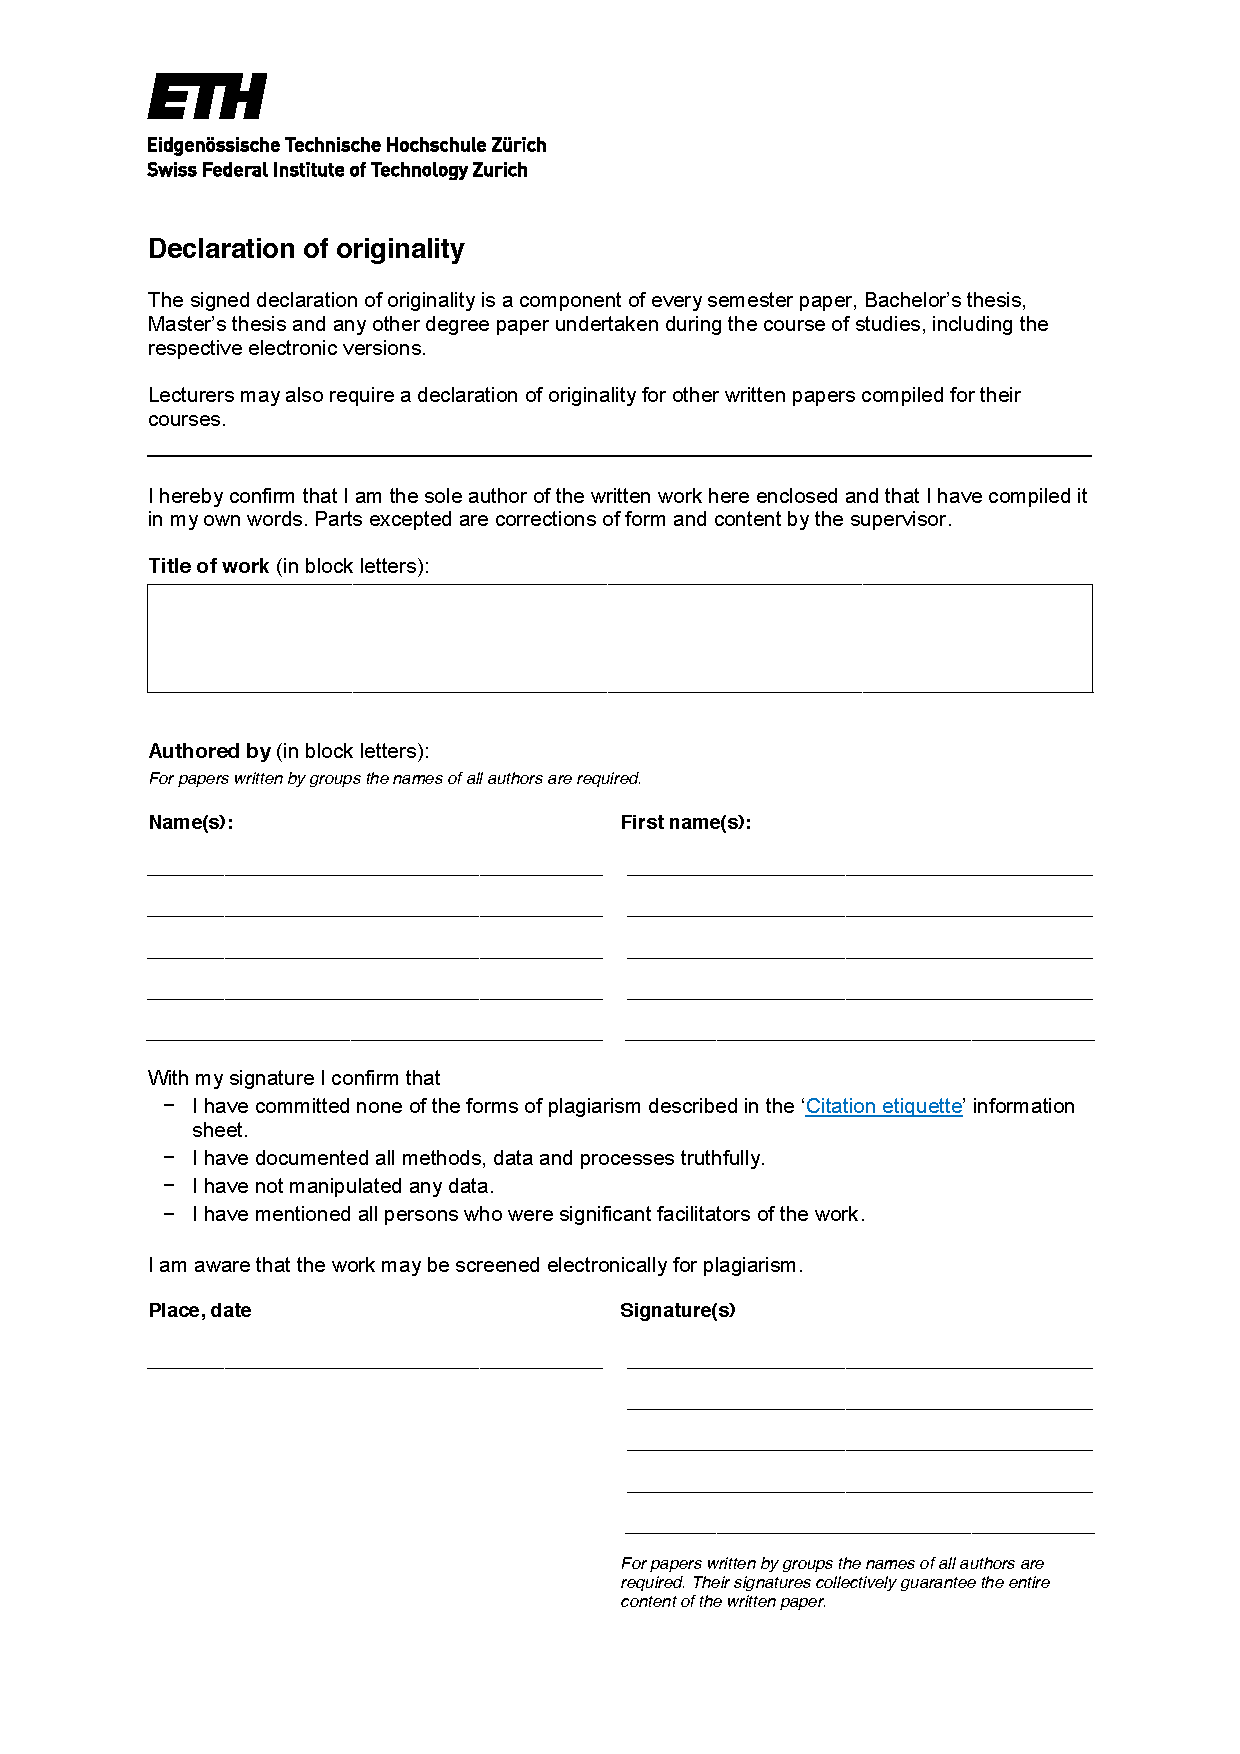
\includepdf[pages={-}]{declaration-originality.pdf}

\end{document}
